% Slides BTL1 — bản tiếng Việt. Dựng PDF: tectonic slides/main-vi.tex
\documentclass[aspectratio=169,11pt]{beamer}
\usepackage{amsmath,amssymb,booktabs,tikz,listings}
\usepackage{fontspec}
\setsansfont{DejaVu Sans}[Scale=0.92]
\setmonofont{DejaVu Sans Mono}[Scale=0.86]
\usetikzlibrary{arrows.meta,positioning,calc}
\definecolor{blue}{HTML}{285BC2}
\definecolor{water}{HTML}{258BD2}
\definecolor{ink}{HTML}{25282D}
\definecolor{muted}{HTML}{646E7B}
\definecolor{red}{HTML}{BA463A}
\setbeamercolor{normal text}{fg=ink,bg=white}
\setbeamercolor{structure}{fg=blue}
\setbeamercolor{frametitle}{fg=blue}
\setbeamercolor{itemize item}{fg=blue}
\setbeamerfont{frametitle}{size=\Large,series=\bfseries}
\setbeamerfont{title}{size=\Huge,series=\bfseries}
\setbeamertemplate{navigation symbols}{}
\setbeamertemplate{itemize item}{\small$\bullet$}
\setbeamertemplate{footline}{\hfill\color{muted}\scriptsize\insertframenumber\,/\,\inserttotalframenumber\hspace{7mm}\vspace{4mm}}
\setbeamersize{text margin left=9mm,text margin right=9mm}
\lstset{basicstyle=\ttfamily\footnotesize,columns=fullflexible,
  keepspaces=true,showstringspaces=false,keywordstyle=\color{blue},
  morekeywords={if,return,for,in,while,push,pop,then,else},aboveskip=5pt}
\newcommand{\src}[1]{\vfill{\tiny\color{muted}#1}}
\newcommand{\pipearm}[3]{\draw[draw=#3,line width=3pt,line cap=round] (#1,#2) -- ++(0.43,0);}
% A tile's integer mask uses N=1, E=2, S=4, W=8.
\newcommand{\tile}[4]{%
  \begin{scope}[shift={(#1,#2)}]
    \draw[gray!25] (-.5,-.5) rectangle (.5,.5);
    \foreach \bit/\dx/\dy in {1/0/0.5,2/0.5/0,4/0/-0.5,8/-0.5/0}{%
      \pgfmathtruncatemacro{\hasport}{mod(floor(#3/\bit),2)}
      \ifnum\hasport=1
        \draw[#4,line width=3.6pt,line cap=round] (0,0)--(\dx,\dy);
      \fi}
  \end{scope}}
\newcommand{\board}[2]{%
  \foreach \mask [count=\idx from 0] in {#1}{%
    \pgfmathtruncatemacro{\col}{mod(\idx,4)}
    \pgfmathtruncatemacro{\row}{-floor(\idx/4)}
    \tile{\col}{\row}{\mask}{#2}}
  \fill[white] (2,-2) circle (.15);
  \fill[blue] (2,-2) circle (.11);}

\begin{document}

% ---------- Trang bìa ----------
\begin{frame}[plain]
\begin{columns}[c,onlytextwidth]
\column{.62\textwidth}
{\color{blue}\Huge\bfseries Pipes \& Light Up}\par\vspace{4mm}
{\Large Giải thuật tìm kiếm cho hai bài toán Logic Puzzle}\par\vspace{7mm}
Nhập môn Trí tuệ nhân tạo --- BTL1 (HK1 2026--2027)\par\vspace{3mm}
\small DFS (mù) + Greedy Best-First (Pipes)\quad$\cdot$\quad DFS + MRV/CP (Light Up)\par\vspace{2mm}
\footnotesize [Nhóm --- thành viên điền tại đây]
\column{.33\textwidth}
\centering
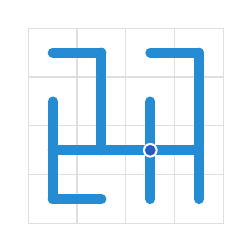
\begin{tikzpicture}[scale=.62]
\board{2,12,2,12,4,5,4,5,7,11,15,13,3,8,1,1}{water}
\end{tikzpicture}
\end{columns}
\end{frame}

% Pipes frames — bản tiếng Việt, được \input từ slides/main-vi.tex.
% Giữ nguyên các lệnh \tile/\board/\src định nghĩa trong preamble của main-vi.tex.

\begin{frame}{Mục tiêu: một mạng liên thông, không chu trình}
\begin{columns}[c,onlytextwidth]
\column{.38\textwidth}\centering
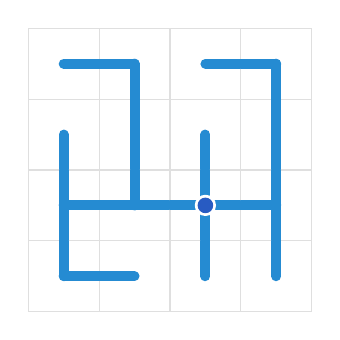
\begin{tikzpicture}[scale=.9]
\board{2,12,2,12,4,5,4,5,7,11,15,13,3,8,1,1}{water}
\end{tikzpicture}
\column{.57\textwidth}
\begin{itemize}
\item Mọi cổng mở đều gặp cổng tương ứng của ô kề.
\item Không cổng nào chìa ra ngoài bàn chơi.
\item Tất cả các ô liên thông. Không có chu trình.
\end{itemize}
\vspace{4mm}
Ô là đỉnh,connections là cạnh:
\[
G\text{ là cây} \quad\Longrightarrow\quad |E|=n-1
\]
\small Nguồn xanh chỉ để trực quan hóa nước chảy.
\end{columns}
\src{Luật: puzzle-pipes.com. Kiểm tra đích: model.py và search.py.}
\end{frame}

\begin{frame}{Phát biểu bài toán tìm kiếm}
\small
\begin{tabular}{@{}p{.23\textwidth}p{.70\textwidth}@{}}
\toprule
Input & $n=m^2$ ô, hình dạng cố định, biên thường (không wrap) \\
Trạng thái & Tiền tố $s=(a_0,\ldots,a_{k-1})$ các định hướng đã gán \\
Trạng thái đầu & Tiền tố rỗng $()$, biết trước mọi hình dạng \\
Tác động & Gán một định hướng cho ô $k$ theo thứ tự row-major \\
Chuyển tiếp & $s'=s+(a_k)$, nhận sau khi qua kiểm tra khả thi \\
Đích & $k=n$ và bàn hoàn chỉnh đạt mọi luật \\
Chi phí & 1 mỗi phép gán; không giải thuật nào dùng để xếp hạng \\
\bottomrule
\end{tabular}\par
\vspace{5mm}
\normalsize Một bước solver có thể tương ứng nhiều lần xoay 90°.\par
\small Mọi lời giải hợp lệ đều chấp nhận; không tối ưu số lần xoay.
\src{Mô hình trạng thái cài đặt: Search trong pipes\_problem/search.py.}
\end{frame}

\begin{frame}{Các successor hợp lệ}
Ô kế tiếp có hình dạng cố định; tìm kiếm chọn định hướng của nó.
\vspace{5mm}
\begin{center}
\begin{tikzpicture}[x=1cm,y=1cm]
\foreach \mask/\x/\label in {3/0/NE,6/3/ES,12/6/SW,9/9/NW}{
  \begin{scope}[shift={(\x,0)}]
    \tile{0}{0}{\mask}{muted}
    \draw[ink,line width=1pt] (.65,.5)--(-.5,.5)--(-.5,-.65);
    \node[below=8mm] at (0,0) {\small\label};
  \end{scope}}
\node[red] at (0,-1.4) {loại};
\node[blue] at (3,-1.4) {giữ};
\node[red] at (6,-1.4) {loại};
\node[red] at (9,-1.4) {loại};
\end{tikzpicture}
\end{center}
\small Ví dụ ô góc trên-trái. Biên trái và trên cấm hướng N và W.\par
\vspace{4mm}
\normalsize Khớp láng giềng cũng kiểm tra cả cổng \emph{không} có.\par
\small Ứng viên phải qua hết các lớp cắt tỉa dùng chung trước khi được nhận.
\src{Ví dụ minh họa. Lọc định hướng: boundary\_domains() và compatible().}
\end{frame}

\begin{frame}{Không gian tìm kiếm}
\begin{columns}[T,onlytextwidth]
\column{.48\textwidth}
\small Số xoay phân biệt mỗi ô\par\vspace{3mm}
\begin{tabular}{@{}lr@{}}\toprule
Khuỷu, chữ T, đầu cụt & 4\\
Ống thẳng & 2\\
Chữ thập & 1\\\bottomrule
\end{tabular}
\vspace{4mm}
\normalsize
\[U=\prod_{i=0}^{n-1}|R_i|\leq 4^n\]
\small Số cách gán đầy đủ, trước kiểm tra biên.
\column{.47\textwidth}
\small Cây tiền tố\par\vspace{3mm}
\begin{tikzpicture}[every node/.style={font=\small},level distance=10mm,
 level 1/.style={sibling distance=24mm},level 2/.style={sibling distance=11mm}]
\node {$()$}
 child {node {$a_0$} child {node {$a_1$}} child {node {$a'_1$}}}
 child {node {$a'_0$} child {node {$\cdots$}}};
\end{tikzpicture}
\par\small Độ sâu $n$, hệ số phân nhánh tối đa 4.\par
Mỗi tiền tố có đúng một cha.
\end{columns}
\vspace{4mm}
Ví dụ 4$\times$4 kèm theo: $U=268{,}435{,}456$.\par
\small Đây là cận trên số cách gán, không phải số node đo được.
\src{Đếm từ các xoay phân biệt trong pipes-4x4-261.json.}
\end{frame}

\begin{frame}{Cắt tỉa dùng chung}
\centering
\begin{tikzpicture}[node distance=5mm,
 test/.style={draw=muted!45,minimum width=95mm,minimum height=7mm,font=\small},
 link/.style={-{Stealth},draw=muted}]
\node[test] (a) {Định hướng hợp lệ biên};
\node[test,below=of a] (b) {Khớp láng giềng đã gán, chặn miền rỗng};
\node[test,below=of b] (c) {Chặn chu trình giữa các ô đã gán};
\node[test,below=of c] (d) {Yêu cầu kết nối khả dĩ của mọi ô};
\draw[link] (a)--(b);\draw[link] (b)--(c);\draw[link] (c)--(d);
\end{tikzpicture}
\vspace{3mm}\par
\small Cả hai giải thuật dùng cùng các kiểm tra và cùng thứ tự ô.\par
\vspace{2mm}
Điều kiện gốc: tổng số cổng $=2(n-1)$.\par
Kết nối khả dĩ là điều kiện cần, chưa chứng minh tồn tại nghiệm.
\src{Cài đặt cắt tỉa: Search.compatible(). Phân tích đầy đủ: docs/pipes-analysis.md.}
\end{frame}

\begin{frame}[fragile]{Tìm kiếm mù: Depth-First Search}
\begin{columns}[T,onlytextwidth]
\column{.60\textwidth}
\begin{lstlisting}
VISIT(s):
  if budget exhausted: return LIMIT
  count expansion
  if GOAL(s): return SOLVED(s)
  for a in rotations of tile |s|:
    child = s + (a)
    if FEASIBLE(child):
      r = VISIT(child)
      if r is SOLVED or LIMIT: return r
  return UNSOLVABLE
\end{lstlisting}
\column{.35\textwidth}
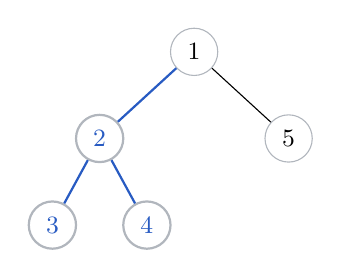
\begin{tikzpicture}[level distance=11mm,
 level 1/.style={sibling distance=24mm},level 2/.style={sibling distance=12mm},
 every node/.style={circle,draw=muted!50,minimum size=6mm,font=\small}]
\node {1}
 child[blue,thick] {node {2} child {node {3}} child {node {4}}}
 child {node {5}};
\end{tikzpicture}
\par\vspace{3mm}\small Thứ tự thăm minh họa.\par
Đi sâu một nhánh rồi quay lui.
\end{columns}
\vspace{4mm}
\small Đầy đủ trên cây hữu hạn với đủ tài nguyên và cắt tỉa hợp lệ.\par
Trường hợp xấu nhất vẫn hàm mũ.
\src{Giả mã rút gọn khớp dfs(). Kiểm tra gốc chạy trước VISIT.}
\end{frame}

\begin{frame}{Heuristic của Greedy: số lựa chọn còn lại}
\[
h(s)=\sum_{i\text{ chưa gán}}\log_2 |D_i(s)|
\]
\small $D_i(s)$ là miền định hướng hợp lệ biên, khớp láng giềng đã gán.
\vspace{5mm}
\begin{center}
\begin{tabular}{@{}lcc@{}}
\toprule
Ứng viên & Kích thước miền còn lại & $h(s)$\\\midrule
A & $(1,2,4)$ & $0+1+2=3$\\
B & $(1,1,2)$ & $0+0+1=1$\\\bottomrule
\end{tabular}
\end{center}
\vspace{3mm}
Greedy ưu tiên B: giá trị nhỏ hơn nghĩa là ít lựa chọn còn lại.\par
\small Thứ tự hòa: tiền tố sâu hơn, rồi tới chèn sớm hơn.\par\vspace{3mm}
Điểm số bỏ qua ràng buộc giữa các ô chưa gán.\par
Không admissible, không đảm bảo tối ưu số lần xoay.
\src{Ví dụ miền giả định. Độ ưu tiên thật: (h, -depth, thứ tự chèn) trong greedy().}
\end{frame}

\begin{frame}[fragile]{Greedy Best-First search}
\begin{columns}[T,onlytextwidth]
\column{.61\textwidth}
\begin{lstlisting}
push () into min-priority queue
while queue is not empty:
  if budget exhausted: return LIMIT
  s = pop minimum-priority state
  count expansion
  if GOAL(s): return SOLVED(s)
  for a in rotations of tile |s|:
    child = s + (a)
    D = FEASIBLE(child)
    if D exists:
      push child with (h(child),
                       -|child|, serial)
return UNSOLVABLE
\end{lstlisting}
\column{.34\textwidth}
\small Chọn từ hàng đợi\par\vspace{3mm}
\begin{tikzpicture}[every node/.style={font=\small}]
\node[draw=blue,minimum width=30mm,minimum height=9mm] (b) {$B:\ h=1$};
\node[below=0mm of b,draw=muted!50,minimum width=30mm,minimum height=9mm] (a) {$A:\ h=3$};
\node[above=6mm of b] (pop) {mở rộng tiếp};
\draw[-{Stealth},blue] (b)--(pop);
\end{tikzpicture}
\par\vspace{3mm}
Mọi tiền tố khả thi đều nằm trong hàng đợi.\par\vspace{3mm}
Bộ nhớ có thể tăng hàm mũ.
\end{columns}
\src{Kiểm tra gốc chạy trước khi push. Độ ưu tiên chỉ dùng h.}
\end{frame}

\begin{frame}{Giao thức đo lường}
\begin{itemize}
\item Cùng 9 map cho cả hai giải thuật.
\item Ba map mỗi kích thước, mỗi giải thuật chạy 5 lượt.
\item Cùng cắt tỉa, cùng thứ tự ô, cùng giới hạn tài nguyên.
\end{itemize}
\vspace{4mm}
\begin{tikzpicture}[every node/.style={font=\small},node distance=17mm]
\node (map) {Map lưu sẵn};
\node[right=of map] (time) {Solve headless, bấm giờ};
\node[right=of time] (mem) {Replay đo bộ nhớ riêng};
\draw[-{Stealth},blue] (map)--(time);
\draw[-{Stealth},blue] (time)--(mem);
\end{tikzpicture}
\vspace{4mm}\par
\small Thời gian không gồm vẽ hình và phát lại. Bộ nhớ là đỉnh cấp phát
Python được trace. Chỉ gộp hai lần đo khi kết quả trùng khớp.\par\vspace{3mm}
Giới hạn: 30 giây tính toán và 200{,}000 lần mở rộng mỗi lượt.
\src{Chạy batch: benchmark.py. Đo: measure() và worker.py.}
\end{frame}

\begin{frame}{Kết quả thực nghiệm}
% Source: docs/benchmarks/2026-10-25-pipes.csv, successful-run group medians (Linux, 25 Oct 2026).
\begin{center}
\small
\begin{tabular}{@{}llrrr@{}}
\toprule
Size & Algorithm & Solved/runs & Time (ms) & Peak (KiB)\\
\midrule
$4\times4$ & DFS    & 15/15 & 3.149  & 26.984\\
           & Greedy & 15/15 & 3.097  & 12.359\\
$5\times5$ & DFS    & 15/15 & 5.261  & 53.297\\
           & Greedy & 15/15 & 6.157  & 19.219\\
$7\times7$ & DFS    & 15/15 & 24.469 & 145.852\\
           & Greedy & 15/15 & 31.695 & 27.594\\
\bottomrule
\end{tabular}
\end{center}

\vspace{3mm}
\small Median trên 15 lượt thành công mỗi kích thước và giải thuật.\par
Mỗi nhóm gồm 3 input phân biệt, 5 lượt bấm giờ.\par\vspace{3mm}
DFS nhanh hơn ở 5$\times$5 và 2/3 map 7$\times$7; Greedy thắng trên map khó nhất
(38.2 so với 40.8\,ms) và giữ bộ nhớ traced thấp hơn 4--5 lần.\par
Input này khá dễ với cắt tỉa hiện có, chưa đủ để kết luận kẻ thắng chung.
\src{Đo ngày 25/10/2026, Linux, Python 3.13. Dữ liệu thô: docs/benchmarks/2026-10-25-pipes.csv.}
\end{frame}

\begin{frame}{Phạm vi và thí nghiệm tiếp theo}
\begin{itemize}
\item Thêm map khó hơn và map vô nghiệm đã chứng minh.
\item Đo riêng đóng góp từng lớp cắt tỉa (ablation).
\item Giữ tách biệt UNSOLVABLE với LIMIT/CANCELLED.
\item Thử heuristic khác (MRV) và mở rộng bộ input.
\end{itemize}
\vspace{5mm}
\small\textbf{Tài liệu tham khảo}\par\vspace{2mm}
Luật Pipes: \url{https://www.puzzle-pipes.com/}\par
Russell \& Norvig, \emph{Artificial Intelligence: A Modern Approach},
4th ed., chương 3 và 6. \url{https://aima.cs.berkeley.edu/}
\end{frame}

% Nội dung Light Up đồng bộ từ submission.tex; dùng định dạng của main-vi.tex.
\begin{frame}{Bài toán 2: Light Up (Akari)}
\begin{columns}[c,onlytextwidth]
\column{.36\textwidth}\centering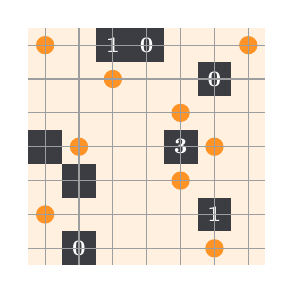
\begin{tikzpicture}[scale=.43]
\fill[orange!12] (-.5,.5) rectangle (6.5,-6.5);
\fill[ink!90] (2-.5,-0-.5) rectangle (2+.5,-0+.5);
\node[white,font=\footnotesize\bfseries] at (2,-0) {1};
\fill[ink!90] (3-.5,-0-.5) rectangle (3+.5,-0+.5);
\node[white,font=\footnotesize\bfseries] at (3,-0) {0};
\fill[ink!90] (5-.5,-1-.5) rectangle (5+.5,-1+.5);
\node[white,font=\footnotesize\bfseries] at (5,-1) {0};
\fill[ink!90] (0-.5,-3-.5) rectangle (0+.5,-3+.5);
\fill[ink!90] (4-.5,-3-.5) rectangle (4+.5,-3+.5);
\node[white,font=\footnotesize\bfseries] at (4,-3) {3};
\fill[ink!90] (1-.5,-4-.5) rectangle (1+.5,-4+.5);
\fill[ink!90] (5-.5,-5-.5) rectangle (5+.5,-5+.5);
\node[white,font=\footnotesize\bfseries] at (5,-5) {1};
\fill[ink!90] (1-.5,-6-.5) rectangle (1+.5,-6+.5);
\node[white,font=\footnotesize\bfseries] at (1,-6) {0};
\fill[orange!85] (0,-0) circle (.27);
\fill[orange!85] (6,-0) circle (.27);
\fill[orange!85] (2,-1) circle (.27);
\fill[orange!85] (4,-2) circle (.27);
\fill[orange!85] (1,-3) circle (.27);
\fill[orange!85] (5,-3) circle (.27);
\fill[orange!85] (4,-4) circle (.27);
\fill[orange!85] (0,-5) circle (.27);
\fill[orange!85] (5,-6) circle (.27);
\draw[ink!45] (-.5,.5) grid (6.5,-6.5);
\end{tikzpicture}

\column{.60\textwidth}\begin{itemize}
\item Đặt bóng trên ô trắng, chiếu theo hàng/cột đến tường.
\item Mọi ô trắng phải sáng.
\item Hai bóng không nhìn thấy nhau.
\item Tường số có đúng số bóng kề trực tiếp.
\end{itemize}\vspace{3mm}
\textbf{Hai giải thuật:} DFS và CSP (backtracking + MRV + CP).
\end{columns}
\src{Luật theo Nikoli. Hình: bàn $7\times7$ seed 70097 và lời giải CSP tìm được.}
\end{frame}

\begin{frame}{Phát biểu bài toán tìm kiếm}
\small\begin{tabular}{@{}p{.22\textwidth}p{.73\textwidth}@{}}\toprule
Thành phần & Biểu diễn\\\midrule
Trạng thái & Tập bóng, ô sáng và vị trí còn hợp lệ (bitmask)\\
Ban đầu & Chưa có bóng; CSP có thể suy ra bóng ngay tại gốc\\
Hành động & Đặt bóng; CSP có thể chọn một tổ hợp quanh tường\\
Đích & Sáng hết ô trắng, không xung đột, mọi số trên tường đúng\\
Không gian & $2^W$ tập bóng trước ràng buộc, với $W$ ô trắng\\\bottomrule
\end{tabular}
\vspace{3mm}\par
Một nút CSP có thể đặt nhiều bóng cùng lúc nhờ suy luận.\par
Cả hai tìm lời giải đầu tiên, không tối ưu số bóng.
\end{frame}

\begin{frame}{Tạo dữ liệu đầu vào}
\begin{enumerate}
\item Dùng seed chọn vị trí tường.
\item Đặt bóng làm chứng đến khi mọi ô trắng sáng.
\item Suy ra số trên tường; giữ một phần tường không số.
\item Kiểm chứng lời giải làm chứng trước khi trả bàn.
\end{enumerate}
\vspace{3mm}\small
4 cỡ: $7,10,14,25$; 3 nhãn; 5 seed khác nhau mỗi cấu hình.\par
Tổng cộng \textbf{60 bản}, mỗi bản dùng chung cho hai giải thuật.
\src{easy/normal/hard khác nhau ở tỉ lệ tường: 16\%, 10.5\%, 5.5\%. Solver không biết lời giải mẫu.}
\end{frame}

\begin{frame}[fragile]{Giải thuật tìm kiếm mù: DFS}
\begin{lstlisting}[breaklines=true]
DFS(state):
  if limit reached: return LIMIT
  if GOAL(state): return SOLVED
  target = first dark cell in row-major order
  for bulb in legal illuminators(target):
    child = place(bulb)
    if FEASIBLE(child):
      result = DFS(child)
      if solved or limited: return result
    exclude bulb from later sibling choices
  return UNSOLVABLE
\end{lstlisting}
\small Đi sâu theo thứ tự cố định. Loại nhánh nếu tường không đủ chỗ hoặc ô tối không còn nguồn chiếu.
\src{Trong code, đệ quy được thay bằng stack tường minh.}
\end{frame}

\begin{frame}{CP: suy luận trước khi chọn nhánh}
\begin{columns}[c,onlytextwidth]
\column{.34\textwidth}\centering
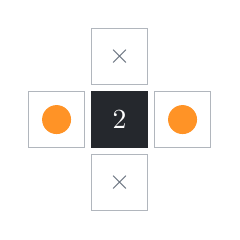
\begin{tikzpicture}[scale=.8]
\foreach \x/\y in {-1/0,1/0,0/1,0/-1}{\draw[muted!50](\x-.45,\y-.45)rectangle(\x+.45,\y+.45);}
\fill[ink](-.45,-.45)rectangle(.45,.45);\node[white]at(0,0){2};
\fill[orange!85](-1,0)circle(.23);\fill[orange!85](1,0)circle(.23);
\node[muted]at(0,1){$\times$};\node[muted]at(0,-1){$\times$};
\end{tikzpicture}\par\vspace{2mm}{\tiny\color{muted}Tường đủ 2 bóng: cấm hai ô kề còn lại.\par}
\column{.62\textwidth}\small
\textbf{\texttt{PROPAGATE}: lặp đến khi không đổi}
\begin{itemize}
\item Tường đủ bóng: cấm các ô kề còn lại.
\item Tường thiếu $r$ bóng, còn đúng $r$ ô: đặt tất cả.
\item Ô tối còn một nguồn chiếu: đặt bóng tại đó.
\item Bóng mới cấm các vị trí nhìn thấy nó; loại ô gây thiếu chỗ quanh tường.
\end{itemize}
\vspace{2mm}Mâu thuẫn $\Rightarrow$ quay lui. Chưa xong $\Rightarrow$ MRV.
\end{columns}
\src{Trạng thái dùng chung: \texttt{(bulbs, lit, legal)} = tập bóng, ô sáng, vị trí còn được phép đặt.}
\end{frame}

\begin{frame}{MRV: chọn ràng buộc có điểm nhỏ nhất}
\begin{columns}[T,onlytextwidth]
\column{.48\textwidth}
\begin{block}{Tường số $w$}
\small $r=k_w-|N(w)\cap bulbs|$: bóng còn thiếu.\par
$u=|N(w)\cap legal|$: ô kề còn được đặt.
\[
 m_{\mathrm{wall}}(w)=\binom{u}{r},\quad r>0
\]
\centering $u=3,\ r=2\ \Rightarrow\ \boxed{m=3}$
\end{block}
\column{.48\textwidth}
\begin{block}{Ô tối $i$}
\small $C(i)=V(i)\cap legal$: các nguồn chiếu.\par
$V(i)$ gồm cả ô $i$.
\[
 m_{\mathrm{dark}}(i)=|C(i)|
\]
\centering Hai nguồn chiếu $\Rightarrow\ \boxed{m=2}$
\end{block}
\end{columns}
\vspace{2mm}\centering
\textbf{Chọn ô tối: $2<3$. Bằng điểm thì ưu tiên tường.}
\src{$N(w)$: ô trắng kề tường; $k_w$: số trên tường. Điểm tường tính trước khi loại tổ hợp bóng chiếu nhau; có thể khác số nhánh thực tế.}
\end{frame}

\begin{frame}{Gain: thử nhánh chiếu sáng thêm nhiều ô trước}
\small Sau khi chọn ràng buộc bằng MRV, xếp nhánh theo
$gain(A)=|(\bigcup_{b\in A}V(b))\cap dark|$ giảm dần.
\begin{columns}[T,onlytextwidth]
\column{.48\textwidth}\centering
\textbf{Nhánh 1: đặt $(7,7)$, gain = 7}\par\vspace{1mm}
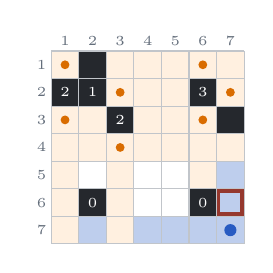
\begin{tikzpicture}[x=.35cm,y=-.35cm,font=\tiny]
% Snapshot after root CP: 7x7 easy, seed 70098; coordinates below are zero-based.
\foreach \c/\r in {0/0,2/0,3/0,4/0,5/0,6/0,2/1,3/1,4/1,6/1,0/2,1/2,3/2,4/2,5/2,0/3,1/3,2/3,3/3,4/3,5/3,6/3,0/4,2/4,5/4,0/5,2/5,0/6,2/6}{\fill[orange!12] (\c,\r) rectangle ++(1,1);}
\foreach \c/\r in {6/4,6/5,1/6,3/6,4/6,5/6,6/6}{\fill[blue!30] (\c,\r) rectangle ++(1,1);}
\foreach \c/\r/\n in {1/0/-1,0/1/2,1/1/1,5/1/3,2/2/2,6/2/-1,1/5/0,5/5/0}{
  \fill[ink] (\c,\r) rectangle ++(1,1);
  \ifnum\n>-1\node[white] at (\c+.5,\r+.5) {\n};\fi}
\foreach \i in {0,...,7}{
  \draw[muted!40,thin] (\i,0)--(\i,7);
  \draw[muted!40,thin] (0,\i)--(7,\i);}
\foreach \c/\r in {0/0,5/0,2/1,6/1,0/2,5/2,2/3}{\fill[orange!85!black] (\c+.5,\r+.5) circle (.16);}
\fill[blue] (6.5,6.5) circle (.22);
\draw[red!80!black,very thick] (6.08,5.08) rectangle (6.92,5.92);
\foreach \i in {0,...,6}{
  \pgfmathtruncatemacro{\labelnum}{\i+1}
  \node[muted] at (\i+.5,-.35) {\labelnum};
  \node[muted] at (-.35,\i+.5) {\labelnum};}
\end{tikzpicture}

\column{.48\textwidth}\centering
\textbf{Nhánh 2: đặt $(5,7)$, gain = 6}\par\vspace{1mm}
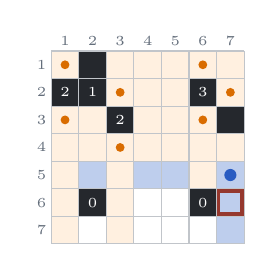
\begin{tikzpicture}[x=.35cm,y=-.35cm,font=\tiny]
% Snapshot after root CP: 7x7 easy, seed 70098; coordinates below are zero-based.
\foreach \c/\r in {0/0,2/0,3/0,4/0,5/0,6/0,2/1,3/1,4/1,6/1,0/2,1/2,3/2,4/2,5/2,0/3,1/3,2/3,3/3,4/3,5/3,6/3,0/4,2/4,5/4,0/5,2/5,0/6,2/6}{\fill[orange!12] (\c,\r) rectangle ++(1,1);}
\foreach \c/\r in {1/4,3/4,4/4,6/4,6/5,6/6}{\fill[blue!30] (\c,\r) rectangle ++(1,1);}
\foreach \c/\r/\n in {1/0/-1,0/1/2,1/1/1,5/1/3,2/2/2,6/2/-1,1/5/0,5/5/0}{
  \fill[ink] (\c,\r) rectangle ++(1,1);
  \ifnum\n>-1\node[white] at (\c+.5,\r+.5) {\n};\fi}
\foreach \i in {0,...,7}{
  \draw[muted!40,thin] (\i,0)--(\i,7);
  \draw[muted!40,thin] (0,\i)--(7,\i);}
\foreach \c/\r in {0/0,5/0,2/1,6/1,0/2,5/2,2/3}{\fill[orange!85!black] (\c+.5,\r+.5) circle (.16);}
\fill[blue] (6.5,4.5) circle (.22);
\draw[red!80!black,very thick] (6.08,5.08) rectangle (6.92,5.92);
\foreach \i in {0,...,6}{
  \pgfmathtruncatemacro{\labelnum}{\i+1}
  \node[muted] at (\i+.5,-.35) {\labelnum};
  \node[muted] at (-.35,\i+.5) {\labelnum};}
\end{tikzpicture}

\end{columns}
\par\vspace{2mm}{\tiny\color{muted}Seed 70098, sau CP ở gốc. Viền đỏ: ô tối $(6,7)$ có hai nguồn chiếu. Chấm cam: bóng đã đặt; chấm xanh: bóng thử; nền xanh: ô mới sáng.\par}
\small\textbf{Thử $(7,7)$ trước $(5,7)$.} Đếm mỗi ô một lần, trước CP của con.
\src{Gain không cộng vào điểm MRV. Nhánh 2 cấm nguồn $(7,7)$ đã thử ở nhánh 1.}
\end{frame}

\begin{frame}[fragile]{Backtracking: CP $\rightarrow$ MRV/gain $\rightarrow$ thử nhánh}
\begin{lstlisting}[breaklines=true]
BACKTRACK_MRV_CP(state):
  if budget exhausted: return LIMIT
  state, ok = PROPAGATE(state)
  if not ok: return UNSOLVABLE
  if GOAL(state): return SOLVED(state)
  checkpoint = state
  choices = SELECT_MRV_CHOICES(checkpoint)
  for child in choices:  # descending gain, before child CP
    result = BACKTRACK_MRV_CP(child)
    if result is SOLVED or LIMIT: return result
    state = checkpoint
  return UNSOLVABLE
\end{lstlisting}
\src{\texttt{SELECT\_MRV\_CHOICES}: chọn ràng buộc, sinh nhánh và xếp gain. Checkpoint giữ đủ \texttt{(bulbs, lit, legal)} sau CP của cha. Code dùng stack thay đệ quy.}
\end{frame}

\begin{frame}{Hiện thực và minh họa từng bước}
\begin{enumerate}
\item Chọn DFS hoặc CSP, bấm Start Search.
\item Pause và hai mũi tên để đi tới/lui từng bước.
\item CSP hiện thêm bóng suy ra, ô bị cấm $\times$ và lúc quay lui.
\item Compare DFS and CSP: chạy cả hai trên bàn đang mở.
\end{enumerate}
\vspace{3mm}\small
Solver chạy trong worker riêng; giao diện nhận từng sự kiện để vẽ.
\src{Python 3, pygame-ce. Luật ở core/, giải thuật ở algorithms/search.py, giao diện ở ui/app.py.}
\end{frame}

\begin{frame}{Kết quả thực nghiệm: số bản giải được}
\centering\small\begin{tabular}{@{}lrrrr@{}}\toprule
 & \multicolumn{2}{c}{DFS} & \multicolumn{2}{c}{CSP}\\
Cỡ & Giải được & TIMEOUT & Giải được & TIMEOUT\\\midrule
$7\times7$ & 15/15 & 0 & 15/15 & 0\\
$10\times10$ & 15/15 & 0 & 15/15 & 0\\
$14\times14$ & 15/15 & 0 & 15/15 & 0\\
$25\times25$ & 7/15 & 8 & 15/15 & 0\\\midrule
Tổng & 52/60 & 8 & 60/60 & 0\\\bottomrule
\end{tabular}\par\vspace{3mm}
\raggedright 60 bản $\times$ 2 giải thuật = 120 lượt. Mỗi bản đo một lần mỗi giải thuật.\par
Giới hạn: 30 giây, 500.000 node, 512 MiB ước lượng.
\src{Mỗi lượt chạy trong process mới. Không lượt nào chạm giới hạn nút hoặc bộ nhớ.}
\end{frame}

% Mean of raw 2026-10-31-lightup-dfs-csp.csv, five seeds per configuration,
% including TIMEOUT; labels give SOLVED counts, not the sample size of each mean.
\begin{frame}{Kết quả: thời lượng trung bình}
\centering
\begin{tikzpicture}[x=.28cm,y=.34cm,font=\scriptsize]
\draw[muted!20] (0.0000,-.1)--(0.0000,10.1);\node[below,muted] at (0.0000,-.1) {0};
\draw[muted!20] (5.0000,-.1)--(5.0000,10.1);\node[below,muted] at (5.0000,-.1) {5};
\draw[muted!20] (10.0000,-.1)--(10.0000,10.1);\node[below,muted] at (10.0000,-.1) {10};
\draw[muted!20] (15.0000,-.1)--(15.0000,10.1);\node[below,muted] at (15.0000,-.1) {15};
\draw[muted!20] (20.0000,-.1)--(20.0000,10.1);\node[below,muted] at (20.0000,-.1) {20};
\draw[muted!20] (25.0000,-.1)--(25.0000,10.1);\node[below,muted] at (25.0000,-.1) {25};
\draw[muted!20] (30.0000,-.1)--(30.0000,10.1);\node[below,muted] at (30.0000,-.1) {30};
\node[anchor=east,align=right] at (-.7,8.65) {14 / easy};
\fill[orange!85!black] (0,9.000) rectangle (0.90696,9.550);
\node[anchor=west,text=orange!85!black] at (1.05696,9.275) {0.9070 (5/5)};
\fill[blue] (0,8.150) rectangle (0.09472,8.700);
\node[anchor=west,text=blue] at (0.24472,8.425) {0.0947 (5/5)};
\node[anchor=east,align=right] at (-.7,5.95) {25 / easy};
\fill[orange!85!black] (0,6.300) rectangle (23.79466,6.850);
\node[anchor=west,text=orange!85!black] at (23.94466,6.575) {23.7947 (2/5)};
\fill[blue] (0,5.450) rectangle (2.10556,6.000);
\node[anchor=west,text=blue] at (2.25556,5.725) {2.1056 (5/5)};
\node[anchor=east,align=right] at (-.7,3.25) {25 / normal};
\fill[orange!85!black] (0,3.600) rectangle (24.29717,4.150);
\node[anchor=west,text=orange!85!black] at (24.44717,3.875) {24.2972 (1/5)};
\fill[blue] (0,2.750) rectangle (1.04439,3.300);
\node[anchor=west,text=blue] at (1.19439,3.025) {1.0444 (5/5)};
\node[anchor=east,align=right] at (-.7,0.55) {25 / hard};
\fill[orange!85!black] (0,0.900) rectangle (7.74997,1.450);
\node[anchor=west,text=orange!85!black] at (7.89997,1.175) {7.7500 (4/5)};
\fill[blue] (0,0.050) rectangle (1.04631,0.600);
\node[anchor=west,text=blue] at (1.19631,0.325) {1.0463 (5/5)};
\draw[muted] (0,-.1)--(30,-.1);
\node[anchor=west,muted] at (30.3,-.1) {giây};
\node[anchor=west,text=orange!85!black] at (0,11) {\rule{3mm}{2mm} DFS};
\node[anchor=west,text=blue] at (6,11) {\rule{3mm}{2mm} CSP};
\node[anchor=east,muted] at (30,11) {Nhãn: mean (số lượt SOLVED/5)};
\end{tikzpicture}
\src{Trung bình cộng trên 5 seed, tính cả TIMEOUT. Đây là thời lượng đến lúc dừng; không phải thời gian giải xong khi có TIMEOUT. Bảng đủ 12 cấu hình nằm trong báo cáo.}
\end{frame}

\begin{frame}{Kết quả: đỉnh bộ nhớ Python trung bình}
\centering
\begin{tikzpicture}[x=.28cm,y=.34cm,font=\scriptsize]
\draw[muted!20] (0.0000,-.1)--(0.0000,10.1);\node[below,muted] at (0.0000,-.1) {0};
\draw[muted!20] (7.5000,-.1)--(7.5000,10.1);\node[below,muted] at (7.5000,-.1) {1000};
\draw[muted!20] (15.0000,-.1)--(15.0000,10.1);\node[below,muted] at (15.0000,-.1) {2000};
\draw[muted!20] (22.5000,-.1)--(22.5000,10.1);\node[below,muted] at (22.5000,-.1) {3000};
\draw[muted!20] (30.0000,-.1)--(30.0000,10.1);\node[below,muted] at (30.0000,-.1) {4000};
\node[anchor=east,align=right] at (-.7,8.65) {14 / easy};
\fill[orange!85!black] (0,9.000) rectangle (1.71653,9.550);
\node[anchor=west,text=orange!85!black] at (1.86653,9.275) {228.9 (5/5)};
\fill[blue] (0,8.150) rectangle (0.81218,8.700);
\node[anchor=west,text=blue] at (0.96218,8.425) {108.3 (5/5)};
\node[anchor=east,align=right] at (-.7,5.95) {25 / easy};
\fill[orange!85!black] (0,6.300) rectangle (16.44688,6.850);
\node[anchor=west,text=orange!85!black] at (16.59688,6.575) {2192.9 (2/5)};
\fill[blue] (0,5.450) rectangle (4.34916,6.000);
\node[anchor=west,text=blue] at (4.49916,5.725) {579.9 (5/5)};
\node[anchor=east,align=right] at (-.7,3.25) {25 / normal};
\fill[orange!85!black] (0,3.600) rectangle (26.41534,4.150);
\node[anchor=west,text=orange!85!black] at (26.56534,3.875) {3522.0 (1/5)};
\fill[blue] (0,2.750) rectangle (5.19749,3.300);
\node[anchor=west,text=blue] at (5.34749,3.025) {693.0 (5/5)};
\node[anchor=east,align=right] at (-.7,0.55) {25 / hard};
\fill[orange!85!black] (0,0.900) rectangle (9.51490,1.450);
\node[anchor=west,text=orange!85!black] at (9.66490,1.175) {1268.7 (4/5)};
\fill[blue] (0,0.050) rectangle (6.54200,0.600);
\node[anchor=west,text=blue] at (6.69200,0.325) {872.3 (5/5)};
\draw[muted] (0,-.1)--(30,-.1);
\node[anchor=west,muted] at (30.3,-.1) {KiB};
\node[anchor=west,text=orange!85!black] at (0,11) {\rule{3mm}{2mm} DFS};
\node[anchor=west,text=blue] at (6,11) {\rule{3mm}{2mm} CSP};
\node[anchor=east,muted] at (30,11) {Nhãn: mean (số lượt SOLVED/5)};
\end{tikzpicture}
\src{Trung bình đỉnh cấp phát Python qua 5 seed, tính cả TIMEOUT; không phải RAM cả process. Cùng tập lượt chạy với biểu đồ thời lượng.}
\end{frame}

\begin{frame}{Nhận xét}
\begin{itemize}
\item CSP giải đủ 60/60 bàn, DFS 52/60; 8 lượt TIMEOUT đều ở bàn $25\times25$.
\item Cỡ 25: số nút DFS khoảng 2\,408--13\,407, CSP khoảng 34--96; mỗi nút CSP có thể suy ra nhiều bóng.
\item Trong 52 cặp cùng giải được: DFS nhanh hơn ở 37 bàn, CSP ở 15 bàn. Chi phí CP có thể lấn lợi ích trên bàn nhỏ.
\end{itemize}
\vspace{3mm}\textbf{Hạn chế:} mỗi cấu hình mới 5 seed; nhãn độ khó chỉ dựa trên số tường; chưa đo riêng tác dụng MRV, gain và CP.
\end{frame}


% ---------- Kết ----------
\begin{frame}{Tổng kết}
\begin{itemize}
\item Pipes: DFS / Greedy. Light Up đo mới: DFS / MRV + CP.
\item Demo đủ bước tìm kiếm; CSP có cả từng suy luận bắt buộc.
\item Light Up: 60 bàn khác nhau, 120 lượt theo cặp, giữ nguyên giới hạn.
\item Ghi tỷ lệ giải được và TIMEOUT / NODE\_LIMIT / MEMORY\_LIMIT riêng.
\item Dữ liệu: \texttt{docs/benchmarks/2026-10-31-lightup-dfs-csp.csv}.
\end{itemize}
\vspace{5mm}
\small\textbf{Tài liệu tham khảo}\par\vspace{2mm}
\url{https://www.puzzle-pipes.com/} $\cdot$ \url{https://www.puzzle-light-up.com/}\par
Russell \& Norvig, \emph{Artificial Intelligence: A Modern Approach}, 4th ed.\par
Cài đặt và phân tích: \texttt{pipes\_problem/}, \texttt{light\_up\_problem/}, \texttt{docs/}.
\end{frame}

\end{document}
